\section{CONDICION IV} 
\textbf{Líneas de investigación a ser desarrolladas}
\vspace{5mm} %5mm vertical space

\vspace{5mm} %5mm vertical space
\begin{center}
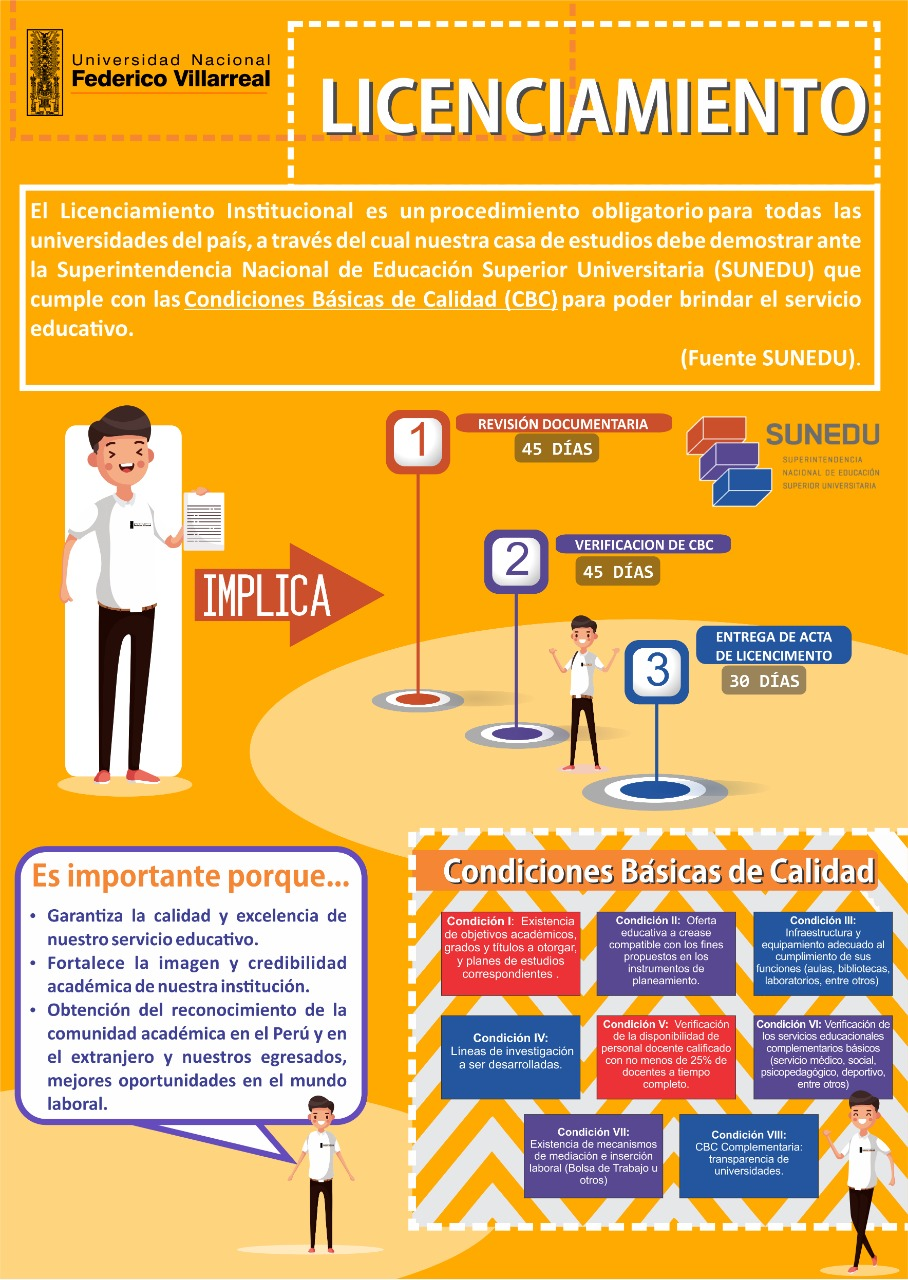
\includegraphics[width=10cm]{./Imagenes/003}
\end{center}	
\vspace{7mm} %3mm vertical space

\textbf{CONDICION IV: Líneas de investigación a ser desarrolladas}\\

-	Son indicadores que corresponden a las líneas de investigación\\
-	Son indicadores que corresponden a docentes que realizan investigación\\ 
-	Son indicadores que corresponden a Registro de documentos y proyectos de investigación.\\
\textbf{CONDICION V: Verificación de la disponibilidad de personal docente calificado con no menos del 25 porciento de docentes a tiempo completo}\\
-	De acuerdo al estatuto vigente de la Universidad Privada de Tacna.\\
\textbf{CONDICION VI: Verificación de los servicios educacionales complementarios básicos (servicio médico, social, psicopedagógico, deportivo, entre otros)}\\
-	Los servicios complementarios básicos con que debe contar mínimamente la universidad son: \\
-	Los servicios complementarios referido a Servicios de salud  \\
-	Los servicios complementarios referido a Servicios culturales  \\
-	Los servicios complementarios referido a Acervo bibliográfico \\
-	Los servicios complementarios referido servicio psicopedagógico\\
 \textbf{CONDICION VII: Existencia de mecanismos de mediación e inserción laboral (Bolsa de Trabajo u otros)}\\
-	Uno de los fines de la Universidad moderna en cuanto a la condición VII\\
-	En la condición VII para que los mecanismos de inserción laboral funcionen\\ 
-	Para el cumplimiento de la condición VII se debe tener en consideración\\
-	La condición VII tiene: CONDICION VIII: CBC complementaria: Transparencia de universidades\\ 
-	Actualmente en el Portal de Transparencia que reglamento(s) de admisión encontramos\\
-         ¿Cuántosi reglamentos de estudiantes actualmente se encuentran en el portal de transparencia?\\ 
-         ¿En el portal de transparencia se encuentran visibles la(s) malla(s) currillar(es) de: \\
-         ¿Cuál es el indicador que corresponde a la Condición Básica de Calidad VIII? \\
-	Es un documento sustentatorio para el medio de verificación MV1 \\
-	Los códigos de los programas de la Escuela Profesional de Contabilidad y Finanzas semipresencial corresponden a:\\ 
-	Los códigos de los programas de la Escuela Profesional de Contabilidad y Finanzas presencial corresponden a: \\
-	Los códigos de los programas de la Escuela Profesional de Administración y sistemas semipresencial corresponden a:\\ 
-	Los códigos de los programas de la Escuela Profesional de Administración y sistemas presencial corresponden a: \\
-	Cuál es el número de cursos generales que tienen los programas de Administración y sistemas – Contabilidad y Finanzas?\
